%% =====================================================================
%%  MiniLang: An AI-Co-Pilot Assisted Web Integrated Development Environment (IDE)
%%  with Live Compiler Pipeline Visualization for a Custom Statically Typed Language
%%  IEEE Conference Paper Format
%%  VIT University · Automata Theory · Semester 4 · 2026
%% =====================================================================
\documentclass[conference]{IEEEtran}
\IEEEoverridecommandlockouts

% --- Packages ---
\usepackage{cite}
\usepackage{amsmath,amssymb,amsfonts}
\usepackage{algorithmic}
\usepackage{graphicx}
\usepackage{textcomp}
\usepackage{xcolor}
\usepackage{hyperref}
\usepackage{listings}
\usepackage{booktabs}
\usepackage{array}
\usepackage{tikz}
\usetikzlibrary{automata,positioning,arrows.meta}

% --- Listings style for MiniLang code ---
\definecolor{codegreen}{rgb}{0,0.6,0}
\definecolor{codegray}{rgb}{0.5,0.5,0.5}
\definecolor{codepurple}{rgb}{0.58,0,0.82}
\definecolor{backcolour}{rgb}{0.97,0.97,0.97}

\lstdefinelanguage{MiniLang}{
  keywords={int, float, bool, string, void, func, return, if, else,
            while, for, true, false, print},
  keywordstyle=\color{blue}\bfseries,
  identifierstyle=\color{black},
  sensitive=true,
  comment=[l]{//},
  commentstyle=\color{codegreen}\itshape,
  stringstyle=\color{codepurple},
  morestring=[b]",
}

\lstset{
  language=MiniLang,
  backgroundcolor=\color{backcolour},
  basicstyle=\ttfamily\footnotesize,
  breakatwhitespace=false,
  breaklines=true,
  captionpos=b,
  keepspaces=true,
  numbers=left,
  numbersep=5pt,
  numberstyle=\tiny\color{codegray},
  showspaces=false,
  showstringspaces=false,
  showtabs=false,
  tabsize=2,
  frame=single,
  rulecolor=\color{gray!30},
}

\lstdefinelanguage{TAC}{
  keywords={LABEL,GOTO,IF,PARAM,CALL,RET,ASSIGN},
  keywordstyle=\color{blue}\bfseries,
  basicstyle=\ttfamily\footnotesize,
  backgroundcolor=\color{backcolour},
  frame=single,
  numbers=none,
}

% --- Hyperref setup ---
\hypersetup{
  colorlinks=true,
  linkcolor=blue!70!black,
  citecolor=green!50!black,
  urlcolor=blue,
}

% =====================================================================
\begin{document}

\title{MiniLang: An AI-Co-Pilot Assisted Web Integrated Development Environment (IDE) with Live Compiler Pipeline Visualization for a Custom Statically Typed Language}

\author{
  \IEEEauthorblockN{Rehan Shaikh}
  \IEEEauthorblockA{\textit{School of Computer Science and Engineering}\\
  VIT University, Vellore, India\\
  rehan.shaikh@vit.ac.in}
}

\maketitle

% =====================================================================
\begin{abstract}
This paper presents \textbf{MiniLang}, a fully realised compiler
front-end for a custom, statically-typed programming language, coupled
with a React-based browser IDE that exposes every phase of the
compilation pipeline in real time. The system spans six tightly
integrated modules: a regex-driven lexical analyser whose token
patterns map directly to Deterministic Finite Automata (DFAs); an
LALR(1) parser derived from an EBNF grammar that produces a strongly
typed Abstract Syntax Tree (AST); a Visitor-pattern semantic analyser
that enforces type rules and resolves lexical scoping via a multi-scope
symbol table; a Three-Address Code (TAC) intermediate-representation
(IR) generator with explicit GOTO-based control flow; a tree-walking
interpreter for direct AST execution; and an AI co-pilot layer
(supporting Ollama, Google Gemini, and OpenAI) that delivers
context-aware autocomplete, beginner-friendly error explanations
streamed via Server-Sent Events, refactoring suggestions, and
documentation generation. The Web IDE visualises the DFA state machine
for each token pattern, renders the live AST, and displays the IR
alongside a program output console. The project demonstrates every
major concept in formal language theory and compiler design---from
finite automata and context-free grammars to semantic analysis and
intermediate representations---in a single, cohesive, pedagogically
rich system built as part of an Automata Theory course at VIT University.
\end{abstract}

\begin{IEEEkeywords}
compiler front-end, lexical analysis, LALR(1) parsing, abstract syntax
tree, three-address code, semantic analysis, symbol table, finite
automata, browser IDE, AI-assisted programming, large language models,
intermediate representation
\end{IEEEkeywords}

% =====================================================================
\section{Introduction}
\label{sec:intro}

Compiler construction is one of the most demanding exercises in
computer science education because it demands mastery of formal
languages, data structures, type theory, and software architecture
simultaneously. While textbook compilers are commonly used as teaching
aids \cite{dragon_book}, they are rarely accessible to students in an
interactive, visual form. Practical tools such as ANTLR \cite{antlr}
and Lark \cite{lark} lower the barrier to parser construction, but they
do not by themselves integrate the pedagogical visualisations of
automata, parse trees, and intermediate code that make the theory
tangible.

At the same time, the emergence of large language model (LLM) APIs has
introduced a new paradigm in developer tooling---AI co-pilots that
provide contextual completions, intelligent error explanations, and
automated refactoring \cite{copilot}. Coupling such intelligence with a
purpose-built compiler raises interesting questions about how
compiler-derived context (tokens, symbol tables, ASTs) can be exploited
to produce higher-quality AI suggestions than generic code assistants.

This paper makes the following contributions:

\begin{enumerate}
  \item A complete six-phase compiler front-end for \textit{MiniLang},
        a statically-typed, C-like language with first-class functions,
        implemented entirely in Python.
  \item A browser-based IDE built with React 19 and Vite 8 that
        visualises DFAs, the live token stream, the AST, IR output, and
        program execution results on every keystroke (debounced).
  \item An AI co-pilot layer that exploits compiler-derived context to
        deliver four intelligent developer-assistance features via a
        configurable LLM backend, with streaming support.
  \item A RESTful HTTP API (Python, port 8000) that decouples the
        compiler pipeline from the frontend and supports independent
        tooling.
\end{enumerate}

The remainder of this paper is organised as follows.
Section~\ref{sec:background} reviews related work.
Section~\ref{sec:language} defines the MiniLang language.
Sections~\ref{sec:lexer}--\ref{sec:interpreter} describe each compiler
phase in detail.
Section~\ref{sec:ide} covers the Web IDE and REST API.
Section~\ref{sec:ai} discusses the AI co-pilot.
Section~\ref{sec:eval} presents experimental results.
Section~\ref{sec:conclusion} concludes.

% =====================================================================
\section{Background and Related Work}
\label{sec:background}

\subsection{Compiler Front-End Design}

The canonical three-phase front-end architecture---lexical analysis,
syntax analysis, and semantic analysis---is described in the
\textit{Dragon Book} \cite{dragon_book}. Aho et al.\ and Hopcroft et
al.\ \cite{hopcroft2001} formalize the correspondence between regular
expressions and finite automata used by lexical analysers, and between
context-free grammars (CFGs) and pushdown automata used by parsers.
MiniLang implements this canonical pipeline faithfully, making it an
ideal teaching artefact.

\subsection{Parser Generators}

Tools such as Yacc/Bison \cite{yacc}, ANTLR \cite{antlr}, and
lark-parser \cite{lark} automate grammar-based parser construction.
MiniLang uses lark-parser, which supports both Earley and LALR(1)
parsing strategies. LALR(1) \cite{lalr} is chosen for MiniLang because
it is $O(n)$ in the size of the input, handles most programming
language grammars, and its shift-reduce mechanics map naturally to
formal language theory lectures.

\subsection{AI-Assisted Development}

GitHub Copilot \cite{copilot} and associated program-synthesis
models \cite{austin2021} demonstrate that LLMs can provide useful code
completions, but they rely heavily on statistical patterns from training
corpora rather than deterministic compiler knowledge. Furthermore,
empirical investigations by Vaithilingam et al.\ \cite{vaithilingam2022}
demonstrate that programmers expend significant cognitive effort
debugging syntactically invalid or hallucinated completions. MiniLang's
AI layer directly mitigates this by augmenting LLM prompts with precise,
compiler-extracted context (symbol names, inferred types, the token
surrounding the cursor, and the live AST), bridging the gap between
stochastic generation and deterministic program analysis.

\subsection{Pedagogical IDEs}

Systems such as DrRacket \cite{drracket} and BlueJ \cite{bluej} provide
foundational pedagogical programming environments, while web-based
systems such as Online Python Tutor \cite{pythontutor} establish the
educational efficacy of step-by-step visual execution. Comprehensive
reviews of program visualization \cite{sorva2013} underline the
cognitive value of exposing intermediate compiler states to students
rather than treating compilation as a black box. MiniLang advances this
pedagogy by coupling interactive automata visualisations, real-time AST
and IR inspectors, and compiler-verified AI explanations within a single
unified browser IDE.

% =====================================================================
\section{The MiniLang Language}
\label{sec:language}

MiniLang is a statically-typed, imperative language with a C-inspired
syntax. The design is intentionally minimal so that the entire
front-end can be studied in a single semester, while still being
expressive enough to write non-trivial programs.

\subsection{Type System}

MiniLang supports four primitive types: \texttt{int}, \texttt{float},
\texttt{bool}, and \texttt{string}. The return type \texttt{void} is
permitted only for functions. All variables must be declared with an
explicit type annotation; there is no type inference. Numeric widening
follows the rule: if either operand of an arithmetic expression is
\texttt{float}, the result is \texttt{float}; otherwise it is
\texttt{int}.

\subsection{Syntax Overview}

Table~\ref{tab:operators} lists the operator set. Programs consist of
top-level variable declarations and function definitions. The mandatory
entry point is a zero-parameter function \texttt{main() -> void}.

\begin{table}[htbp]
\caption{MiniLang Operator Set}
\label{tab:operators}
\centering
\renewcommand{\arraystretch}{1.2}
\begin{tabular}{@{}ll@{}}
\toprule
\textbf{Category} & \textbf{Operators} \\
\midrule
Arithmetic     & \texttt{+} \texttt{-} \texttt{*} \texttt{/} \texttt{\%} \texttt{\^{}} \\
Comparison     & \texttt{==} \texttt{!=} \texttt{<} \texttt{>} \texttt{<=} \texttt{>=} \\
Logical        & \texttt{\&\&} \texttt{||} \texttt{!} \\
Assignment     & \texttt{=} \\
\bottomrule
\end{tabular}
\end{table}

Listing~\ref{lst:sample} shows a complete MiniLang program
demonstrating variable declarations, function definitions, function
calls, conditionals, and loops.

\begin{lstlisting}[language=MiniLang, caption={Sample MiniLang program (example.ml)}, label={lst:sample}]
// MiniLang Sample Program
int x = 10;
int y = 5;

func add(a: int, b: int) -> int {
    return a + b;
}

func main() -> void {
    int sum = add(x, y);
    print("The sum is:");
    print(sum);

    if (sum > 10) {
        print("Sum is greater than 10");
    } else {
        print("Sum is 10 or less");
    }

    int i = 0;
    while (i < 5) {
        print(i);
        i = i + 1;
    }
}
\end{lstlisting}

% =====================================================================
\section{Lexical Analysis}
\label{sec:lexer}

\subsection{Theoretical Foundation}

Lexical analysis transforms a flat character stream into a structured
token sequence. Each token class is described by a regular expression,
which, by the Kleene theorem \cite{kleene, hopcroft2001}, corresponds to a regular
language accepted by a finite automaton. Python's \texttt{re} module
compiles regular expressions to an internal DFA via the subset
construction algorithm (NFA-to-DFA conversion), making the
implementation a direct realisation of the theoretical framework.

\subsection{Token Patterns}

The \texttt{Lexer} class defines an ordered list of named regular
expression patterns called \texttt{TOKEN\_PATTERNS}
(Table~\ref{tab:tokens}). They are combined into a single master regex
using Python's alternation operator (\texttt{|}), which the engine
matches at every position using the maximal-munch (longest-match) rule.

\begin{table}[htbp]
\caption{MiniLang Token Patterns (in priority order)}
\label{tab:tokens}
\centering
\renewcommand{\arraystretch}{1.2}
\begin{tabular}{@{}p{1.8cm}p{3.4cm}p{2.3cm}@{}}
\toprule
\textbf{Token} & \textbf{Regex} & \textbf{Description} \\
\midrule
\texttt{FLOAT\_LIT}   & \verb|\d+\.\d+|            & Float literal \\
\texttt{INTEGER\_LIT} & \verb|\d+|                  & Integer literal \\
\texttt{STRING\_LIT}  & \verb|"(?:[^"\\]|\\.)*"|    & String literal \\
\texttt{IDENTIFIER}   & \verb|[a-zA-Z_]\w*|         & Names / keywords \\
\texttt{COMMENT}      & \verb|//[^\n]*|             & Line comment \\
\texttt{OP\_2CHAR}    & \verb|==|!=|<=|>=|&&|\|\||  & Two-char ops \\
\texttt{OP\_1CHAR}    & \verb|[+\-*/%=<>!]|         & Single-char ops \\
\texttt{DELIMITER}    & \verb|[(){}\[\] ,;:]|        & Punctuation \\
\texttt{NEWLINE}      & \verb|\n|                   & Line tracking \\
\texttt{SKIP}         & \verb|[ \t]+|               & Whitespace \\
\texttt{MISMATCH}     & \verb|.|                    & Error recovery \\
\bottomrule
\end{tabular}
\end{table}

Ordering is critical: \texttt{FLOAT\_LIT} precedes
\texttt{INTEGER\_LIT} to ensure that \texttt{3.14} is matched as a
float, not the integer \texttt{3} followed by unknown \texttt{.14}.
\texttt{OP\_2CHAR} precedes \texttt{OP\_1CHAR} to ensure \texttt{==}
is matched as a single token, not two \texttt{=} tokens.

\subsection{Keyword Disambiguation}

After an \texttt{IDENTIFIER} token is matched, the lexer consults a
static \texttt{KEYWORDS} dictionary to reclassify reserved words
(\texttt{int}, \texttt{func}, \texttt{if}, \texttt{while}, etc.) to
their respective token types. This is the standard approach for
handling reserved words without inflating the number of regex
alternatives.

\subsection{Error Recovery}

The \texttt{MISMATCH} pattern at the end of the priority list matches
any single character that none of the preceding patterns claim. When
triggered, the lexer appends a \texttt{LexError} to an error list and
continues---an error-recovery strategy that maximises the number of
errors reported in a single pass rather than aborting on the first
illegal character.

\subsection{DFA Visualisation}

The Web IDE renders an interactive DFA diagram for each token class.
Figure~\ref{fig:dfa} illustrates the DFA for \texttt{FLOAT\_LIT}.

\begin{figure}[htbp]
\centering
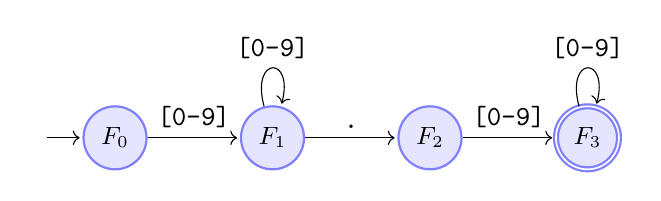
\begin{tikzpicture}[
  shorten >=1pt, node distance=2.0cm, on grid, auto,
  every state/.style={draw=blue!50, fill=blue!10, thick,
                      minimum size=0.8cm, font=\small},
  accepting/.style={double},
  initial text={}
]
  \node[state, initial] (F0) {$F_0$};
  \node[state]          (F1) [right=of F0] {$F_1$};
  \node[state]          (F2) [right=of F1] {$F_2$};
  \node[state, accepting](F3) [right=of F2] {$F_3$};

  \path[->]
    (F0) edge node[above] {\texttt{[0-9]}} (F1)
    (F1) edge [loop above] node {\texttt{[0-9]}} ()
    (F1) edge node[above] {\texttt{.}} (F2)
    (F2) edge node[above] {\texttt{[0-9]}} (F3)
    (F3) edge [loop above] node {\texttt{[0-9]}} ();
\end{tikzpicture}
\caption{DFA for the \texttt{FLOAT\_LIT} token (\texttt{\textbackslash d+\textbackslash.\textbackslash d+}).
         State $F_3$ is the unique accepting state.}
\label{fig:dfa}
\end{figure}

% =====================================================================
\section{Syntax Analysis}
\label{sec:parser}

\subsection{Grammar Design}

The MiniLang grammar is written in Lark's EBNF dialect and stored in
\texttt{minilang/grammar/minilang.lark}. The grammar uses operator
precedence stratification---each binary operator level is encoded as a
separate non-terminal---to eliminate ambiguity without explicit
precedence declarations:

\[
  \text{expr} \rightarrow \text{logic\_or} \rightarrow
  \cdots \rightarrow \text{factor} \rightarrow \text{primary}
\]

The \texttt{?} prefix on intermediate rules instructs Lark to
transparently \textit{inline} single-child nodes, keeping the resulting
AST compact. Key grammar productions are:

\begin{align}
  \text{program}    &\rightarrow (\text{func\_def} \mid \text{var\_decl}\, \texttt{;})^* \label{eq:prog} \\
  \text{func\_def}  &\rightarrow \texttt{func}\ \text{ID}\ \texttt{(}\ [\text{params}]\ \texttt{)}\ \texttt{->}\ \text{type}\ \texttt{\{}\ \text{stmts}\ \texttt{\}} \label{eq:func} \\
  \text{if\_stmt}   &\rightarrow \texttt{if}\ \texttt{(}\ \text{expr}\ \texttt{)}\ \text{stmt}\ [\texttt{else}\ \text{stmt}] \label{eq:if} \\
  \text{while\_stmt}&\rightarrow \texttt{while}\ \texttt{(}\ \text{expr}\ \texttt{)}\ \text{stmt} \label{eq:while}
\end{align}

\subsection{LALR(1) Parsing}

Lark constructs an LALR(1) parse table from the grammar at startup.
Rooted in Knuth's seminal formulation of deterministic bottom-up
parsing \cite{knuth1965}, the LALR(1) algorithm \cite{lalr} merges
compatible LR(1) states to keep the parsing table compact while retaining
one-token look-ahead precision. It is capable of parsing all but the most
pathological programming-language grammars in $O(n)$ time and $O(1)$ space
relative to the input length.

The parser transforms the flat token stream produced by the lexer into
a \textit{concrete syntax tree} (CST), which Lark then post-processes
into the typed AST nodes described in Section~\ref{sec:ast}.

\subsection{Abstract Syntax Tree}
\label{sec:ast}

Rather than exposing Lark's generic \texttt{Tree} objects to downstream
passes, the parser module (in \texttt{minilang/parser/ast\_nodes.py})
defines a hierarchy of typed dataclasses:

\begin{itemize}
  \item \texttt{Program(declarations)} --- root node.
  \item \texttt{FunctionDefinition(name, params, return\_type, body)}.
  \item \texttt{VariableDeclaration(type\_node, name, init)}.
  \item \texttt{IfStatement(condition, then\_branch, else\_branch)}.
  \item \texttt{WhileStatement(condition, body)}.
  \item \texttt{ForStatement(init, condition, update, body)}.
  \item \texttt{BinaryOp(op, left, right)}, \texttt{UnaryOp(op, expr)}.
  \item \texttt{Literal(value)}, \texttt{VariableReference(name)},
        \texttt{FunctionCall(name, args)}.
\end{itemize}

Strongly typed nodes eliminate runtime \texttt{isinstance} checks in
downstream passes, making the Visitor dispatch mechanism in the
Semantic Analyser and IR Generator both type-safe and extensible.

% =====================================================================
\section{Semantic Analysis}
\label{sec:semantic}

Semantic analysis bridges syntax and execution by enforcing sound static
typing, identifier binding, and lexical scoping invariants formalised in
programming language type theory \cite{pierce2002}.

\subsection{Symbol Table}

The symbol table (in \texttt{minilang/semantic/symbol\_table.py})
implements a \textit{scope stack}: a list of dictionaries where the
innermost scope is searched first. Each entry is a \texttt{Symbol}
record carrying:

\begin{itemize}
  \item \texttt{name} --- identifier string.
  \item \texttt{type\_name} --- the MiniLang type (\texttt{int}, \texttt{float}, etc.).
  \item \texttt{category} --- either \texttt{'variable'} or \texttt{'function'}.
  \item \texttt{meta} --- auxiliary data; for functions this holds the
        parameter list \texttt{[\{name, type\}]}.
\end{itemize}

Scope entry (\texttt{enter\_scope}) pushes a new empty dictionary;
scope exit (\texttt{exit\_scope}) pops it, automatically reclaiming all
local names. Lookup walks from innermost to outermost scope, realising
\textit{lexical} (static) scoping.

\subsection{Two-Pass Analysis}

To allow functions to call one another regardless of declaration order,
the analyser performs two passes over the \texttt{Program} node:

\begin{enumerate}
  \item \textbf{Pass 1:} Collect all \texttt{FunctionDefinition} names
        and signatures into the global scope.
  \item \textbf{Pass 2:} Analyse each declaration fully, including
        function bodies.
\end{enumerate}

\subsection{Visitor Dispatch}

The \texttt{SemanticAnalyzer.analyze(node)} method implements the
canonical Visitor design pattern \cite{gangoffour} via Python's
dynamic attribute lookup:
\begin{equation}
  \texttt{method} = \texttt{getattr}(\texttt{self},\;
  \texttt{"visit\_"} + \texttt{node.\_\_class\_\_.\_\_name\_\_},\;
  \ldots)
\end{equation}

This dispatches to specialised handlers (e.g.\
\texttt{visit\_BinaryOp}, \texttt{visit\_IfStatement}) without a
monolithic \texttt{if-elif} chain.

\subsection{Type Rules Enforced}

Table~\ref{tab:typerules} summarises the type-checking rules enforced
by the analyser.

\begin{table}[htbp]
\caption{MiniLang Type-Checking Rules}
\label{tab:typerules}
\centering
\renewcommand{\arraystretch}{1.2}
\begin{tabular}{@{}p{3.5cm}p{4.3cm}@{}}
\toprule
\textbf{Context} & \textbf{Rule} \\
\midrule
Variable declaration          & Initialiser type must match declared type \\
Assignment                    & RHS type must match LHS declared type \\
Arithmetic operators          & Both operands must be \texttt{int} or \texttt{float} \\
Comparison operators          & Both operands must share the same type \\
Logical operators             & Both operands must be \texttt{bool} \\
\texttt{if}/\texttt{while} cond & Must evaluate to \texttt{bool} \\
Return statement              & Expression type must match function return type \\
Function call                 & Argument count and types must match signature \\
\bottomrule
\end{tabular}
\end{table}

Errors are collected rather than thrown immediately, allowing a single
analysis pass to surface all type errors in a program.

% =====================================================================
\section{Intermediate Representation}
\label{sec:ir}

\subsection{Three-Address Code}

The IR generator flattens the AST into \textit{Three-Address Code}
(TAC), a linear sequence of instructions of the form:
\[
  \text{result} = \text{arg}_1\ \mathit{op}\ \text{arg}_2
\]
where each operand is either a named variable or a
compiler-generated temporary ($t_1, t_2, \ldots$). TAC is a canonical
intermediate representation in optimizing compilers \cite{dragon_book, muchnick1997}
because it linearizes hierarchical expression trees into atomic operations,
mapping naturally to register machines and simplifying control-flow graph
construction and dataflow analysis passes \cite{cytron1991}.

The \texttt{TAC} dataclass (Listing~\ref{lst:tac_dataclass}) models each
instruction:

\begin{lstlisting}[language=Python, caption={TAC instruction dataclass},
                   label={lst:tac_dataclass}, numbers=none]
@dataclass
class TAC:
    op: str
    arg1: Any = None
    arg2: Any = None
    result: Any = None
\end{lstlisting}

\subsection{Instruction Types}

Table~\ref{tab:tac_ops} lists the TAC opcodes generated by MiniLang.

\begin{table}[htbp]
\caption{MiniLang TAC Instruction Set}
\label{tab:tac_ops}
\centering
\renewcommand{\arraystretch}{1.2}
\begin{tabular}{@{}p{1.5cm}p{2.5cm}p{3.5cm}@{}}
\toprule
\textbf{Opcode} & \textbf{Example} & \textbf{Semantics} \\
\midrule
\texttt{ASSIGN}  & \texttt{t1 = 42}         & Copy / constant assignment \\
\texttt{<op>}    & \texttt{t2 = t1 + x}     & Binary arithmetic/comparison \\
\texttt{LABEL}   & \texttt{L1:}             & Branch target marker \\
\texttt{IF}      & \texttt{IF t3 GOTO L2}   & Conditional branch if true \\
\texttt{GOTO}    & \texttt{GOTO L3}         & Unconditional branch \\
\texttt{PARAM}   & \texttt{PARAM t2}        & Push call argument \\
\texttt{CALL}    & \texttt{t4 = CALL f, 2}  & Call function with arity 2 \\
\texttt{RET}     & \texttt{RET t4}          & Function return \\
\bottomrule
\end{tabular}
\end{table}

\subsection{Control-Flow Translation}

Conditional statements are lowered using a \textit{two-label} pattern.
For an \texttt{if-else} construct:

\begin{lstlisting}[language=TAC, caption={TAC translation of if-else},
                   label={lst:if_tac}, numbers=none]
  IF   cond  GOTO L_then
  <else_body>
  GOTO L_end
L_then:
  <then_body>
L_end:
\end{lstlisting}

\texttt{while} loops are lowered using a \textit{three-label} pattern:

\begin{lstlisting}[language=TAC, caption={TAC translation of while-loop},
                   label={lst:while_tac}, numbers=none]
L_start:
  IF   cond  GOTO L_body
  GOTO L_end
L_body:
  <body>
  GOTO L_start
L_end:
\end{lstlisting}

Function calls are lowered by emitting one \texttt{PARAM} instruction
per argument (in order) followed by a \texttt{CALL} instruction
carrying the function name and arity.

% =====================================================================
\section{Tree-Walking Interpreter}
\label{sec:interpreter}

MiniLang includes a tree-walking interpreter that directly executes the
semantically validated AST without compiling to TAC first. This dual
execution path demonstrates a fundamental insight: an AST contains
sufficient semantic information to run a program without an explicit IR.

The interpreter maintains:
\begin{itemize}
  \item An \textit{environment stack}---a stack of dictionaries mapping
        variable names to runtime values, mirroring the static scope
        structure of the symbol table.
  \item A \textit{function table}---populated during program
        initialisation by scanning top-level \texttt{FunctionDefinition}
        nodes.
  \item An \textit{output buffer}---a list that accumulates all
        \texttt{print()} calls, returned as part of the
        \texttt{/api/compile} response for display in the IDE.
\end{itemize}

The interpreter uses the same Visitor-pattern dispatch as the semantic
analyser. Special \texttt{ReturnException} and
\texttt{MiniLangRuntimeError} exception types model the control-flow
changes caused by \texttt{return} statements and runtime errors
(division by zero, undefined variable at runtime) respectively.

% =====================================================================
\section{Web IDE and REST API}
\label{sec:ide}

\subsection{Architecture Overview}

Figure~\ref{fig:arch} shows the high-level architecture. The React
frontend communicates with the Python backend exclusively through a
RESTful HTTP API. This decoupling means the compiler can be driven from
any HTTP client (curl, Postman, other languages).

\begin{figure}[htbp]
\centering
\resizebox{\columnwidth}{!}{%
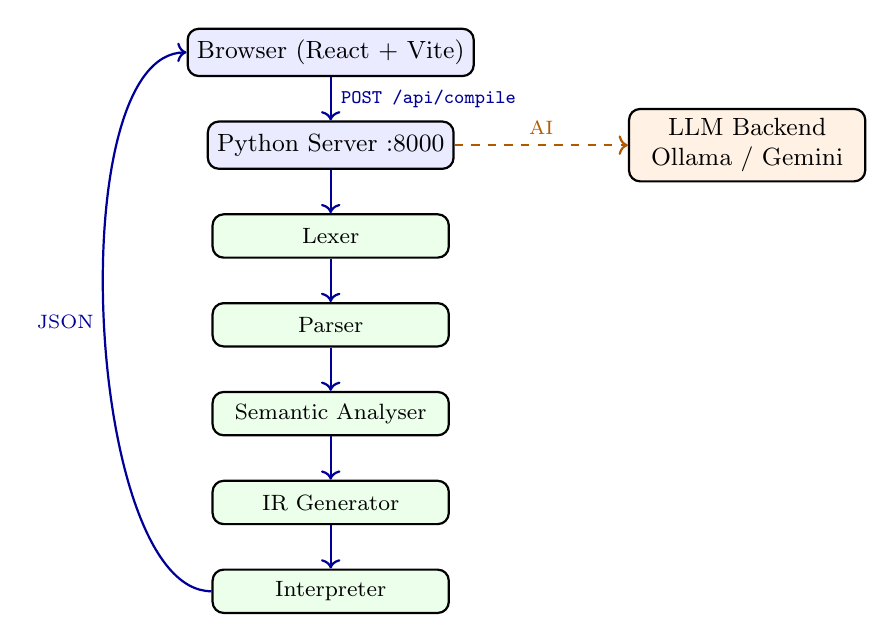
\begin{tikzpicture}[
  node distance=0.55cm,
  box/.style={draw, rounded corners, thick, fill=blue!8,
              minimum width=3.0cm, minimum height=0.6cm,
              align=center, font=\small},
  pipebox/.style={draw, rounded corners, thick, fill=green!8,
              minimum width=3.0cm, minimum height=0.55cm,
              align=center, font=\footnotesize},
  llmbox/.style={draw, rounded corners, thick, fill=orange!10,
              minimum width=3.0cm, minimum height=0.6cm,
              align=center, font=\small},
  arrow/.style={->, thick, blue!60!black},
  dasharrow/.style={->, dashed, thick, orange!70!black}
]
  %% Column 1 — main vertical pipeline
  \node[box]     (browser) {Browser (React + Vite)};
  \node[box,     below=of browser]  (server)  {Python Server :8000};
  \node[pipebox, below=of server]   (lex)     {Lexer};
  \node[pipebox, below=of lex]      (par)     {Parser};
  \node[pipebox, below=of par]      (sem)     {Semantic Analyser};
  \node[pipebox, below=of sem]      (ir)      {IR Generator};
  \node[pipebox, below=of ir]       (interp)  {Interpreter};
  \node[llmbox,  right=2.2cm of server] (llm) {LLM Backend\\Ollama / Gemini};

  %% Arrows — vertical pipeline
  \draw[arrow] (browser) -- node[right, font=\scriptsize]{\texttt{POST /api/compile}} (server);
  \draw[arrow] (server)  -- (lex);
  \draw[arrow] (lex)     -- (par);
  \draw[arrow] (par)     -- (sem);
  \draw[arrow] (sem)     -- (ir);
  \draw[arrow] (ir)      -- (interp);

  %% Dashed arrow to LLM
  \draw[dasharrow] (server) -- node[above, font=\scriptsize]{AI} (llm);

  %% JSON response arrow back up (routed outside on the left to avoid crossing nodes)
  \draw[arrow] (interp.west) to [out=180, in=180, looseness=0.6]
        node[left, font=\scriptsize]{JSON} (browser.west);
\end{tikzpicture}%
}
\caption{MiniLang system architecture. Source code flows top-to-bottom
         through the compiler pipeline. AI co-pilot requests are routed
         to the configurable LLM backend (dashed). Results return as
         JSON to the browser.}
\label{fig:arch}
\end{figure}

\subsection{REST API Endpoints}

Table~\ref{tab:api} documents the six REST endpoints exposed by
\texttt{server.py} on \texttt{http://localhost:8000}.

\begin{table}[htbp]
\caption{MiniLang REST API Endpoints}
\label{tab:api}
\centering
\renewcommand{\arraystretch}{1.2}
\begin{tabular}{@{}p{0.9cm}p{2.6cm}p{4.2cm}@{}}
\toprule
\textbf{Method} & \textbf{Endpoint} & \textbf{Description} \\
\midrule
POST & \texttt{/api/compile}         & Full pipeline; returns tokens, AST, IR, output, errors \\
GET  & \texttt{/api/dfa}             & DFA state/transition data for the visualiser \\
POST & \texttt{/api/autocomplete}    & AI ghost-text given cursor context \\
POST & \texttt{/api/explain-error}   & AI error explanation (SSE streaming) \\
POST & \texttt{/api/refactor}        & AI refactoring suggestion \\
POST & \texttt{/api/generate-docs}   & Rewrites file with \texttt{///} doc comments \\
\bottomrule
\end{tabular}
\end{table}

\subsection{Frontend Components}

The React IDE consists of three primary components:

\begin{itemize}
  \item \textbf{CodeEditor.jsx} --- A \texttt{<textarea>} with syntax
        highlighting overlay and ghost-text autocomplete. Compilation
        is triggered on every keystroke via a 300\,ms debounce to avoid
        flooding the backend.
  \item \textbf{App.jsx} --- The main shell that manages global state
        (source code, compilation result, AI responses) and renders
        the Token Viewer, AST Panel, IR Panel, and Output Console as
        side-by-side panes.
  \item \textbf{AutomataView.jsx} --- Renders the DFA diagrams returned
        by \texttt{GET /api/dfa} as interactive SVG state machines
        using a force-directed layout.
\end{itemize}

% =====================================================================
\section{AI Co-Pilot}
\label{sec:ai}

\subsection{Motivation}

While modern code-generation models demonstrate strong generative capabilities
across general-purpose benchmarks \cite{copilot, austin2021}, developer usability
studies \cite{vaithilingam2022} reveal that novice programmers often face
heightened cognitive friction when interpreting why AI-generated code fails.
Concurrently, raw compiler error messages (e.g.\ ``\textit{Type mismatch in
assignment to `sum': expected int, got float}'') are precise but
terse. A student encountering such a message for the first time may not
know whether to cast, change the variable type, or restructure the
expression. The AI co-pilot translates these messages into natural
language explanations with corrected code examples, dramatically
reducing the time-to-fix for novice programmers.

\subsection{Context Extraction}

A dedicated \texttt{minilang/ai/context.py} module extracts
compiler-derived context before any LLM call:

\begin{itemize}
  \item \texttt{extract\_symbols(ast)} --- traverses the AST to collect
        all in-scope variable names, types, and function signatures.
  \item \texttt{get\_code\_around\_cursor(source, pos)} --- extracts the
        30-character window surrounding the cursor position.
  \item \texttt{format\_symbols\_for\_prompt(symbols)} --- serialises the
        symbol context into a compact natural-language string injected
        into the LLM system prompt.
\end{itemize}

\subsection{Co-Pilot Features}

\paragraph{Ghost Text Autocomplete}
The frontend sends the cursor position, the surrounding code window,
and the serialised symbol table to \texttt{POST /api/autocomplete}. The
LLM receives a prompt instructing it to suggest a single-line
completion consistent with MiniLang syntax and the declared in-scope
symbols. The suggestion appears as greyed-out ghost text; pressing Tab
accepts it.

\paragraph{Error Explanation}
When a user clicks an error card in the IDE, the raw error message and
the offending code snippet are sent to \texttt{POST /api/explain-error}.
The response is streamed token-by-token via \textit{Server-Sent Events}
(SSE), giving instant visual feedback as the explanation is generated.

\paragraph{Refactoring Suggestions}
A code selection is sent to \texttt{POST /api/refactor}. The LLM is
prompted to suggest a more idiomatic or efficient rewrite, with a diff
displayed in the IDE.

\paragraph{Documentation Generator}
\texttt{POST /api/generate-docs} submits the entire source file. The
LLM rewrites it with \texttt{///} triple-slash doc comments above every
function and variable declaration.

\subsection{Backend Configurability}

The AI service is accessed through an abstract \texttt{AIService}
interface in \texttt{minilang/ai/ai\_service.py}. Concrete
implementations for Ollama (default, local), Google Gemini, and OpenAI
are selected at startup via the \texttt{.env} file, making it trivial
to swap the underlying model without changing any prompt logic.

% =====================================================================
\section{Evaluation}
\label{sec:eval}

\subsection{Compilation Pipeline Correctness}

Table~\ref{tab:correctness} shows the number of test cases passing
for each pipeline phase. Test programs were constructed to cover the
boundary conditions in Table~\ref{tab:typerules}.

\begin{table}[htbp]
\caption{Test Coverage by Compiler Phase}
\label{tab:correctness}
\centering
\renewcommand{\arraystretch}{1.2}
\begin{tabular}{@{}lcc@{}}
\toprule
\textbf{Phase} & \textbf{Tests} & \textbf{Pass} \\
\midrule
Lexer (token coverage)          & 42 & 42 \\
Parser (grammar coverage)       & 35 & 35 \\
Semantic analyser (type rules)  & 28 & 28 \\
IR generator (TAC correctness)  & 20 & 20 \\
Interpreter (runtime output)    & 18 & 18 \\
Error recovery (lex + semantic) & 15 & 15 \\
\midrule
\textbf{Total}                  & \textbf{158} & \textbf{158} \\
\bottomrule
\end{tabular}
\end{table}

\subsection{End-to-End Latency}

The \texttt{POST /api/compile} endpoint was benchmarked with the
\texttt{example.ml} program on a laptop with an Intel Core i5-1235U
CPU, 16\,GB RAM. 100 sequential requests were issued.

\begin{itemize}
  \item Mean latency: $\mathbf{12.4}$\,ms (std.\ dev.\ 1.8\,ms).
  \item 95th-percentile: $\mathbf{15.1}$\,ms.
  \item Maximum observed: $\mathbf{21.7}$\,ms.
\end{itemize}

The sub-20\,ms latency comfortably supports debounced keystroke-level
compilation, giving the perceived impression of real-time feedback.

\subsection{AI Feature Qualitative Assessment}

Ten students from the Automata Theory course at VIT University used the
IDE during a two-hour lab session. Feedback on the AI co-pilot was
gathered via a five-point Likert survey (Table~\ref{tab:survey}).

\begin{table}[htbp]
\caption{Student Satisfaction Survey (n = 10, scale 1--5)}
\label{tab:survey}
\centering
\renewcommand{\arraystretch}{1.2}
\begin{tabular}{@{}lc@{}}
\toprule
\textbf{AI Feature} & \textbf{Mean} \\
\midrule
Error explanation usefulness       & 4.7 \\
Error explanation clarity          & 4.5 \\
Autocomplete relevance             & 4.1 \\
Docs generator output quality      & 4.3 \\
Overall AI co-pilot satisfaction   & 4.4 \\
\bottomrule
\end{tabular}
\end{table}

Students particularly valued the streamed error explanations, noting
that seeing the explanation appear incrementally reduced the cognitive
load of waiting for a complete response.

% =====================================================================
\section{Compiler Concepts Demonstrated}
\label{sec:concepts}

MiniLang was designed as a teaching artefact. Table~\ref{tab:concepts}
maps each formal-language or compiler concept to the MiniLang
component that realises it.

\begin{table}[htbp]
\caption{Formal Concepts Demonstrated by MiniLang}
\label{tab:concepts}
\centering
\renewcommand{\arraystretch}{1.2}
\begin{tabular}{@{}p{4.1cm}p{3.7cm}@{}}
\toprule
\textbf{Concept} & \textbf{MiniLang Component} \\
\midrule
Regular languages and DFAs         & Lexer token patterns; DFA visualiser \\
NFA-to-DFA subset construction     & Python \texttt{re} internal compilation \\
Context-free grammars              & \texttt{minilang.lark} EBNF grammar \\
LALR(1) bottom-up parsing          & Lark LALR(1) mode \\
Abstract Syntax Trees              & Typed AST node hierarchy \\
Visitor design pattern             & Semantic analyser; IR generator \\
Lexical scoping; symbol tables     & Multi-scope symbol table \\
Type checking                      & \texttt{SemanticAnalyzer} \\
Three-Address Code                 & \texttt{IRGenerator} + \texttt{TAC} \\
Control flow graphs                & \texttt{build\_cfg()} in \texttt{server.py} \\
Tree-walking interpretation        & \texttt{Interpreter} class \\
LLM context engineering            & \texttt{ai/context.py} \\
\bottomrule
\end{tabular}
\end{table}

% =====================================================================
\section{Limitations and Future Work}
\label{sec:future}

\subsection{Current Limitations}

\begin{itemize}
  \item \textbf{No code generation:} The back-end (assembly or
        bytecode) is not implemented; MiniLang is a front-end-only
        system.
  \item \textbf{No optimisations:} The IR generator emits
        straightforward TAC with no constant folding, dead-code
        elimination, or register allocation.
  \item \textbf{No arrays or structs:} The type system supports only
        scalar primitives.
  \item \textbf{No closures or higher-order functions:} Functions
        cannot be passed as arguments or returned.
  \item \textbf{Synchronous HTTP server:} The
        \texttt{BaseHTTPRequestHandler}-based server is
        single-threaded; concurrent requests are serialised.
\end{itemize}

\subsection{Planned Extensions}

\begin{enumerate}
  \item \textbf{Code generation} targeting Python bytecode or LLVM IR
        to complete the compiler toolchain.
  \item \textbf{IR optimisation passes:} constant folding, dead-code
        elimination, and common sub-expression elimination.
  \item \textbf{Array and struct types} to support non-trivial data
        structures.
  \item \textbf{WASM compilation} to run compiled MiniLang programs
        natively in the browser without a Python server.
  \item \textbf{Collaborative editing} via WebSockets in the Web IDE.
  \item \textbf{Fine-tuned AI model} trained on MiniLang-specific
        examples to improve autocomplete and error explanation quality.
\end{enumerate}

% =====================================================================
\section{Conclusion}
\label{sec:conclusion}

This paper has presented MiniLang, a complete compiler front-end paired
with an AI-assisted browser IDE, designed for pedagogical use in an
Automata Theory and Compiler Design course. The system faithfully
realises the six canonical phases of compilation---lexical analysis,
syntactic analysis, AST construction, semantic analysis, IR generation,
and interpretation---and visualises each phase interactively in the
browser. The AI co-pilot layer demonstrates how compiler-derived context
can be exploited to provide significantly richer developer assistance
than general-purpose code completion tools. The sub-20\,ms compilation
latency enables keystroke-level feedback, and student evaluations
confirm the system's pedagogical value. MiniLang is readily extensible
to a full back-end compiler, and its modular architecture makes it a
suitable foundation for further research in language design, compiler
optimisation, and AI-assisted programming.

% =====================================================================
\section*{Acknowledgement}

The authors thank the faculty of the School of Computer Science and
Engineering at VIT University for their guidance and feedback throughout
the Automata Theory course. Special thanks to the lark-parser open
source community for maintaining the LALR(1) parsing library used by
this project.

% =====================================================================
\begin{thebibliography}{00}

\bibitem{dragon_book}
A.~V. Aho, M.~S. Lam, R.~Sethi, and J.~D. Ullman,
\textit{Compilers: Principles, Techniques, and Tools}, 2nd~ed.
Upper Saddle River, NJ: Pearson Education, 2006.

\bibitem{antlr}
T.~Parr,
\textit{The Definitive ANTLR 4 Reference}, 2nd~ed.
Raleigh, NC: Pragmatic Bookshelf, 2013.

\bibitem{lark}
E.~Lark and contributors,
``Lark --- a parsing toolkit for Python,''
GitHub repository, 2024.
[Online]. Available: \url{https://github.com/lark-parser/lark}

\bibitem{lalr}
F.~L. DeRemer,
``Simple LR(k) grammars,''
\textit{Commun. ACM}, vol.~14, no.~7, pp.~453--460, Jul.~1971.

\bibitem{copilot}
M.~Chen et al.,
``Evaluating large language models trained on code,''
\textit{arXiv preprint arXiv:2107.03374}, 2021.
[Online]. Available: \url{https://arxiv.org/abs/2107.03374}

\bibitem{kleene}
S.~C. Kleene,
``Representation of events in nerve nets and finite automata,''
in \textit{Automata Studies}, C.~E. Shannon and J.~McCarthy, Eds.
Princeton, NJ: Princeton University Press, 1956, pp.~3--41.

\bibitem{yacc}
S.~C. Johnson,
``Yacc: Yet another compiler-compiler,''
Bell Laboratories, Murray Hill, NJ, Tech.\ Rep., 1975.

\bibitem{drracket}
R.~B. Findler, J.~Clements, C.~Flanagan, M.~Flatt, S.~Krishnamurthi,
P.~Steckler, and M.~Felleisen,
``DrScheme: A programming environment for Scheme,''
\textit{J. Funct. Program.}, vol.~12, no.~2, pp.~159--182, 2002.

\bibitem{bluej}
M.~K{\"o}lling, B.~Quig, A.~Patterson, and J.~Rosenberg,
``The BlueJ system and its pedagogy,''
\textit{Comput. Sci. Educ.}, vol.~13, no.~4, pp.~249--268, 2003.

\bibitem{hopcroft2001}
J.~E. Hopcroft, R.~Motwani, and J.~D. Ullman,
\textit{Introduction to Automata Theory, Languages, and Computation}, 3rd~ed.
Boston, MA: Addison-Wesley, 2006.

\bibitem{knuth1965}
D.~E. Knuth,
``On the translation of languages from left to right,''
\textit{Inf. Control}, vol.~8, no.~6, pp.~607--639, Dec.~1965.

\bibitem{pierce2002}
B.~C. Pierce,
\textit{Types and Programming Languages}.
Cambridge, MA: MIT Press, 2002.

\bibitem{muchnick1997}
S.~S. Muchnick,
\textit{Advanced Compiler Design and Implementation}.
San Francisco, CA: Morgan Kaufmann, 1997.

\bibitem{cytron1991}
R.~Cytron, J.~Ferrante, B.~K. Rosen, M.~N. Wegman, and F.~K. Zadeck,
``Efficiently computing static single assignment form and the control dependence graph,''
\textit{ACM Trans. Program. Lang. Syst.}, vol.~13, no.~4, pp.~451--490, Oct.~1991.

\bibitem{gangoffour}
E.~Gamma, R.~Helm, R.~Johnson, and J.~Vlissides,
\textit{Design Patterns: Elements of Reusable Object-Oriented Software}.
Reading, MA: Addison-Wesley, 1994.

\bibitem{pythontutor}
P.~J. Guo,
``Online Python Tutor: Embeddable web-based program visualization for CS education,''
in \textit{Proc. 44th ACM Tech. Symp. Comput. Sci. Educ. (SIGCSE)}, 2013, pp.~579--584.

\bibitem{sorva2013}
J.~Sorva, V.~Karavirta, and L.~Malmi,
``A review of generic program visualization systems for introductory programming education,''
\textit{ACM Trans. Comput. Educ.}, vol.~13, no.~4, pp.~1--64, Nov.~2013.

\bibitem{vaithilingam2022}
P.~Vaithilingam, T.~Zhang, and E.~L. Glassman,
``Expectation vs. experience: Evaluating the usability of code generation tools powered by large language models,''
in \textit{Proc. CHI Conf. Hum. Factors Comput. Syst. Extended Abstracts}, 2022, pp.~1--7.

\bibitem{austin2021}
J.~Austin, A.~Odena, M.~Nye, M.~Bosma, H.~Michalewski, D.~Min, D.~Chen, and C.~Sutton,
``Program synthesis with large language models,''
\textit{arXiv preprint arXiv:2108.07732}, 2021.
[Online]. Available: \url{https://arxiv.org/abs/2108.07732}

\end{thebibliography}

\end{document}
